\documentclass{article}
\usepackage[screen]{geometry}
\usepackage{alltt,xcolor}
\usepackage[utf8]{inputenc}
\usepackage{listings}
\usepackage{graphicx}
\usepackage{hyperref}
\lstset{escapechar=\@,language=C++,keywordstyle=\color{blue},showstringspaces=false}
\begin{document}
\normalsize 
\section*{Specification}
calculate the distance traveled by an object over some period 
of seconds when it is dropped based on gravity.





The equation for the distance traveled by a freely falling object is  
$y = \frac{1}{2}gt^2$, where t is time in seconds 
and g is the acceleration of gravity near the surface of the Earth, 
$g = 9.8 \frac{m}{s^2}$. Notice that this equation is 
independent of the mass of the object.

Create a program that outputs a sentence expressing the distance traveled in the given time. For example, an input of 10 seconds should have the output sentence “After the first 10 seconds, the object has fallen 490 meters.”
\newpage\section*{Analysis}

\begin{description}
	\item [inputs]
	How many seconds
	\item [process] Using the gravitational constant.
	The maximus possible distance
	it can travel would be based how high it is dropped from.
	
	\item [outputs]
	The distance traveled.
\end{description}
Reference: 
\href{http://scienceprimer.com/gravitational-acceleration}{Gravitational Acceleration}
\newpage\section*{Design}

\begin{itemize}
	\item Create a constant for the gravitational acceleration.
	\[ 9.8 m/s^{2} \]
	\item acceleration due to gravity is 9.8 m/s2.
	This means that an object, such as a ball, dropped from a small
	distance above the ground will accelerate towards the fround at
	9.8 m/s2. Tf the ball starts with a velocity of zero, it will be
	traveling at 9.8 m/s2 after falling for one second.
	\item $a= \frac{2d}{t^{2}}$ where a is acceleration, t is time in
	seconds, and d is distance. Slove for d :
	\[ d = \frac{at^{2}}{2}  \]
	\item Display the distance to the nearest tenth.
\end{itemize}
\newpage\section*{Implementation}
\lstinputlisting{lab.cpp}
\newpage\section*{Test}
\subsection*{Testcase 1}
For example if the user types in 1 (second),
\[ 4.9 = \frac{9.8 \times 1^{2}}{2} \]then the program will display:
After the 1st second, the object has fallen 4.9 meters
\newline
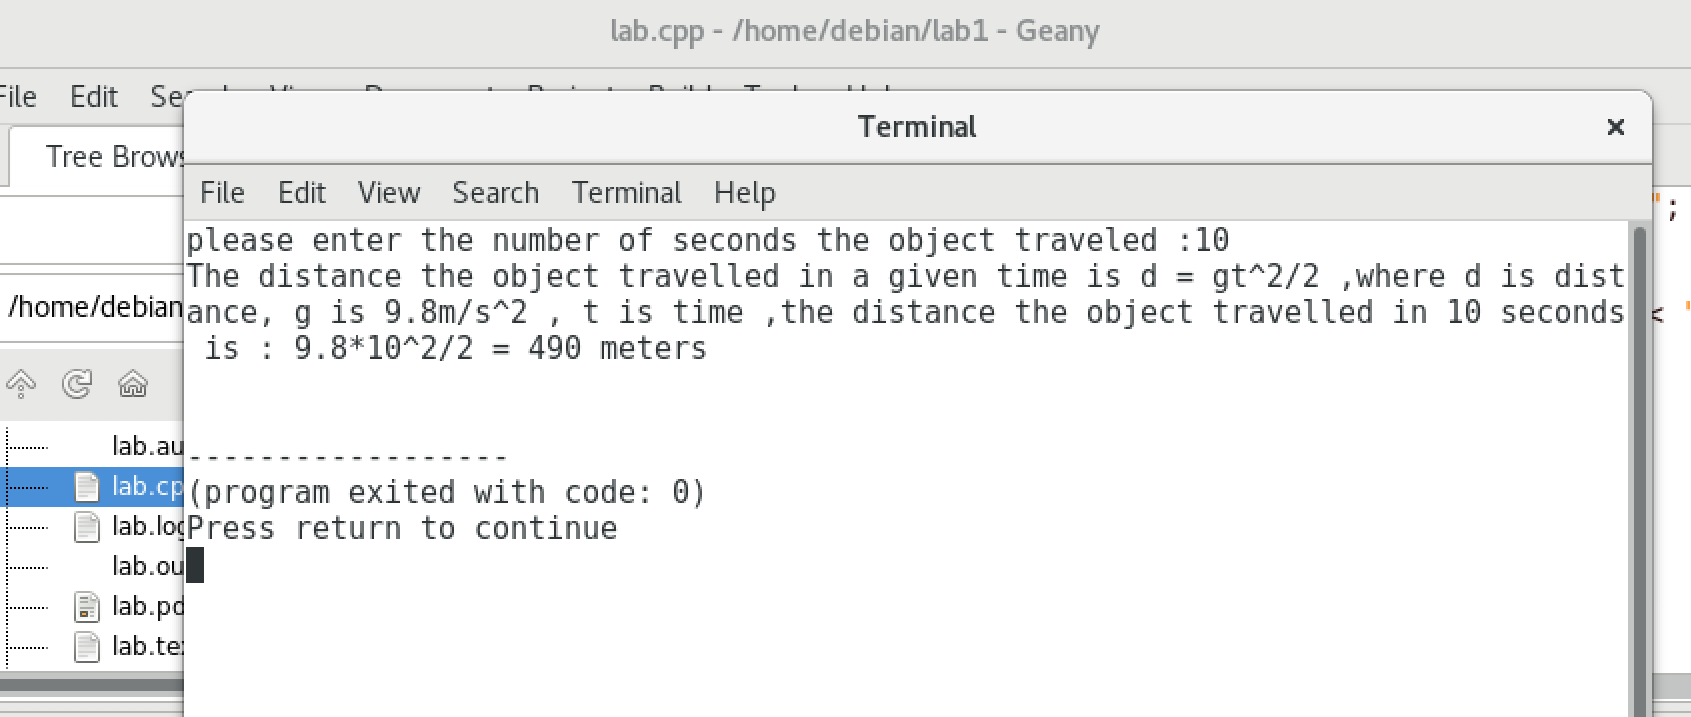
\includegraphics{lab1.png}
\subsection*{Testcase 2}
For example if the user types in 2 (seconds),
\[ 19.6 = \frac{9.8 \times 1^{2}}{2} \],then the program will display:
After the 2 seconds, the object has fallen 19.6 meters
%\includegraphics{testcase2.png}
\end{document}
